In the interstellar medium, many reaction occur, in photon dominated regions (PDR's), as these are the regions where both atomic ions and molecules would coexist. At low temperatures, the rate constant of ion-dipole reactions increase, while other rates decrease or do not change, meaning ion-molecule reaction dominate in these cold (10 K - 100 K) PDR's. In particular, we are interested in the cold production of the formyl isomers (\ce{HCO+ / HOC+}) via \ce{C+} and \ce{H2O}.

\begin{align}
	\ce{C+ + H2O & -> HCO+ + H} \label{r: C+H2O->HCO} \\
	\ce{& -> HOC+ + H} \label{r: C+H2O->HOC} \\
	\ce{HCO+ + H2O & -> H3O+ + CO} \label{r: HCO+H2O->H3O} \\
	\ce{HOC+ + H2O & -> H3O+ + CO} \label{r: HOC+H2O->H3O}
\end{align}

Of which, we verify that the rates of reactions \ref{r: HCO+H2O->H3O} and \ref{r: HOC+H2O->H3O} are indistinguishable in figure \ref{fig: [HCO]+H2O rate} such that we may instead write:

\begin{equation}
	\ce{[HCO]+ + H2O -> H3O+ + CO} \label{r: [HCO]+H2O->H3O}
\end{equation}

Where \ce{[HCO]+} is used to represent both isomers. 

By definition, these formyl isomers of reactions \cref{r: C+H2O->HCO,r: C+H2O->HOC} have identical mass and thus, cannot be readily read off by the TOF system. To be able to separate the isomer products, we need to be able to separate their masses. By introducing a gas into the system with a proton affinity in between the isomer products, we may selectively react only one the less stable \ce{HOC+} isomer. This also yields a distinct $m/z$ peaks originating from separate isomers as seen in reactions \ref{r: X+HOC->XH} and \ref{r: X+HCO->NR}. But by using an external gas, we are doing an indirect measurement, and as such, it may add unintended complications. Certain gasses are more reactive and may react with the excited \ce{Be+}, \ce{C+}, or any other ionized species in the trap. Another possibility is that the \ce{COH+} may isomerize due to interactions with the gas as shown in reaction \ref{r: X+HOC->HCO}.\cite{Love1987}

\begin{align}
	\ce{HOC+ + X & -> XH+ + CO} \label{r: X+HOC->XH} \\
	\ce{& -> HCO+ + X} \label{r: X+HOC->HCO} \\
	\ce{HCO+ + X & -> no reaction} \label{r: X+HCO->NR}
\end{align}

\begin{table}[H]
	\centering
	\label{tab: affinities}
	\begin{tabular}{|l|c|}
	\hline
 & Affinity (kcal/mol)   \\
 \hline
	\ce{CO}* & 427               \\
	\ce{Kr}  & 425               \\
	\ce{HF}  & 490               \\
	\ce{N2}  & 495               \\
	\ce{Xe}  & 496               \\
	\ce{NO}  & 531               \\
	\ce{CO2} & 548               \\
	\ce{CH4} & 552               \\
	\ce{HCl} & 564               \\
	\ce{HBr} & 569               \\
	\ce{N2O} & 571               \\
	*\ce{CO} & 594 \\
	\hline
	\end{tabular}
	\caption{Proton affinities of gasses between formyl isomers where (*) indicates H bonding location.}
\end{table}

Since all reaction products are contained in the trap and continuously exposed to the neutral reactants, we need to consider the possibility that rate constants for reactions \ref{r: HCO+H2O->H3O} and \ref{r: HOC+H2O->H3O} are different. Theoretically, the differing dipole moments of the isomers would produce different dipole-dipole interactions with \ce{H2O} ($C_3$). Literature shows that averaged dipole moments for \ce{HCO+} and \ce{HOC+} are 4.6 D and 2.4 D, respectively.\cite{Rogers1982} The theoretical total rate constants for these reactions are the sum of both ADO and dipole-dipole interaction rates (\ref{eq: k ADO} + \ref{eq: k DD}). Without averaging the dipole oriented angles for the dipole-dipole case, we would have maximal rates of $k_{\ref{r: C+H2O->HCO}} = 8.0 \times 10^{-9}$ cm$^3$/s and $k_{\ref{r: C+H2O->HOC}} = 7.0 \times 10^{-9}$ cm$^3$/s.

We cannot deterministically measure the rate of reaction \ref{r: HOC+H2O->H3O} because there is not a way to produce only \ce{HOC+}, but we may produce only \ce{HCO+}. Considering reactions \ref{r: X+HOC->HCO} and \ref{r: X+HOC->XH}, if we let \ce{X = CO}, we find that both reactions can only yield \ce{HCO+}, allowing us to deterministically produce one of the isomers:

\begin{equation}
\ce{HOC+ + CO -> HCO+ + CO} \label{r: HOC+CO->HCO}
\end{equation}

By producing only \ce{HCO+}, we directly observe \ref{r: HCO+H2O->H3O} with a multi-step reaction procedure. With loaded \ce{Be+} and \ce{C+}, the trap is exposed to \ce{H2O} from the CBGB, to produce a combination of the isomers \ce{[HCO]+}, all the while, \ce{CO} is introduced via the leak valve in the differential cross region to a pressure of $\approx 4 \times 10^{-9}$ Torr as measured in the trap chamber. After $\approx 10$ s of exposure to the CBGB beam, the water beam is shuttered and the trap is exposed to the \ce{CO} for an additional 5 s to ensure full conversion of \ce{HOC+ -> HCO+}, after which, the leak valve is closed. The CBGB is then unshuttered so that the pure \ce{HCO+} is exposed to \ce{H2O} again. The second exposure of the trap to the CBGB defines the reaction time seen in Figure \ref{fig: HCO+H2O rate}. A simpler procedure of continuously exposing the trap to the CBGB yields a combination of the rates of reactions \ref{r: HCO+H2O->H3O} and \ref{r: HOC+H2O->H3O} seen in Figure \ref{fig: [HCO]+H2O rate}.

\todo[inline]{write about the beam density determination with BeOH+}

The respective rates are found with least-squares fitting of the solutions to differential equations found in section \ref{sec: C+H2O eqs}.

The resultant rate constants are 

\begin{figure}
	\centering
	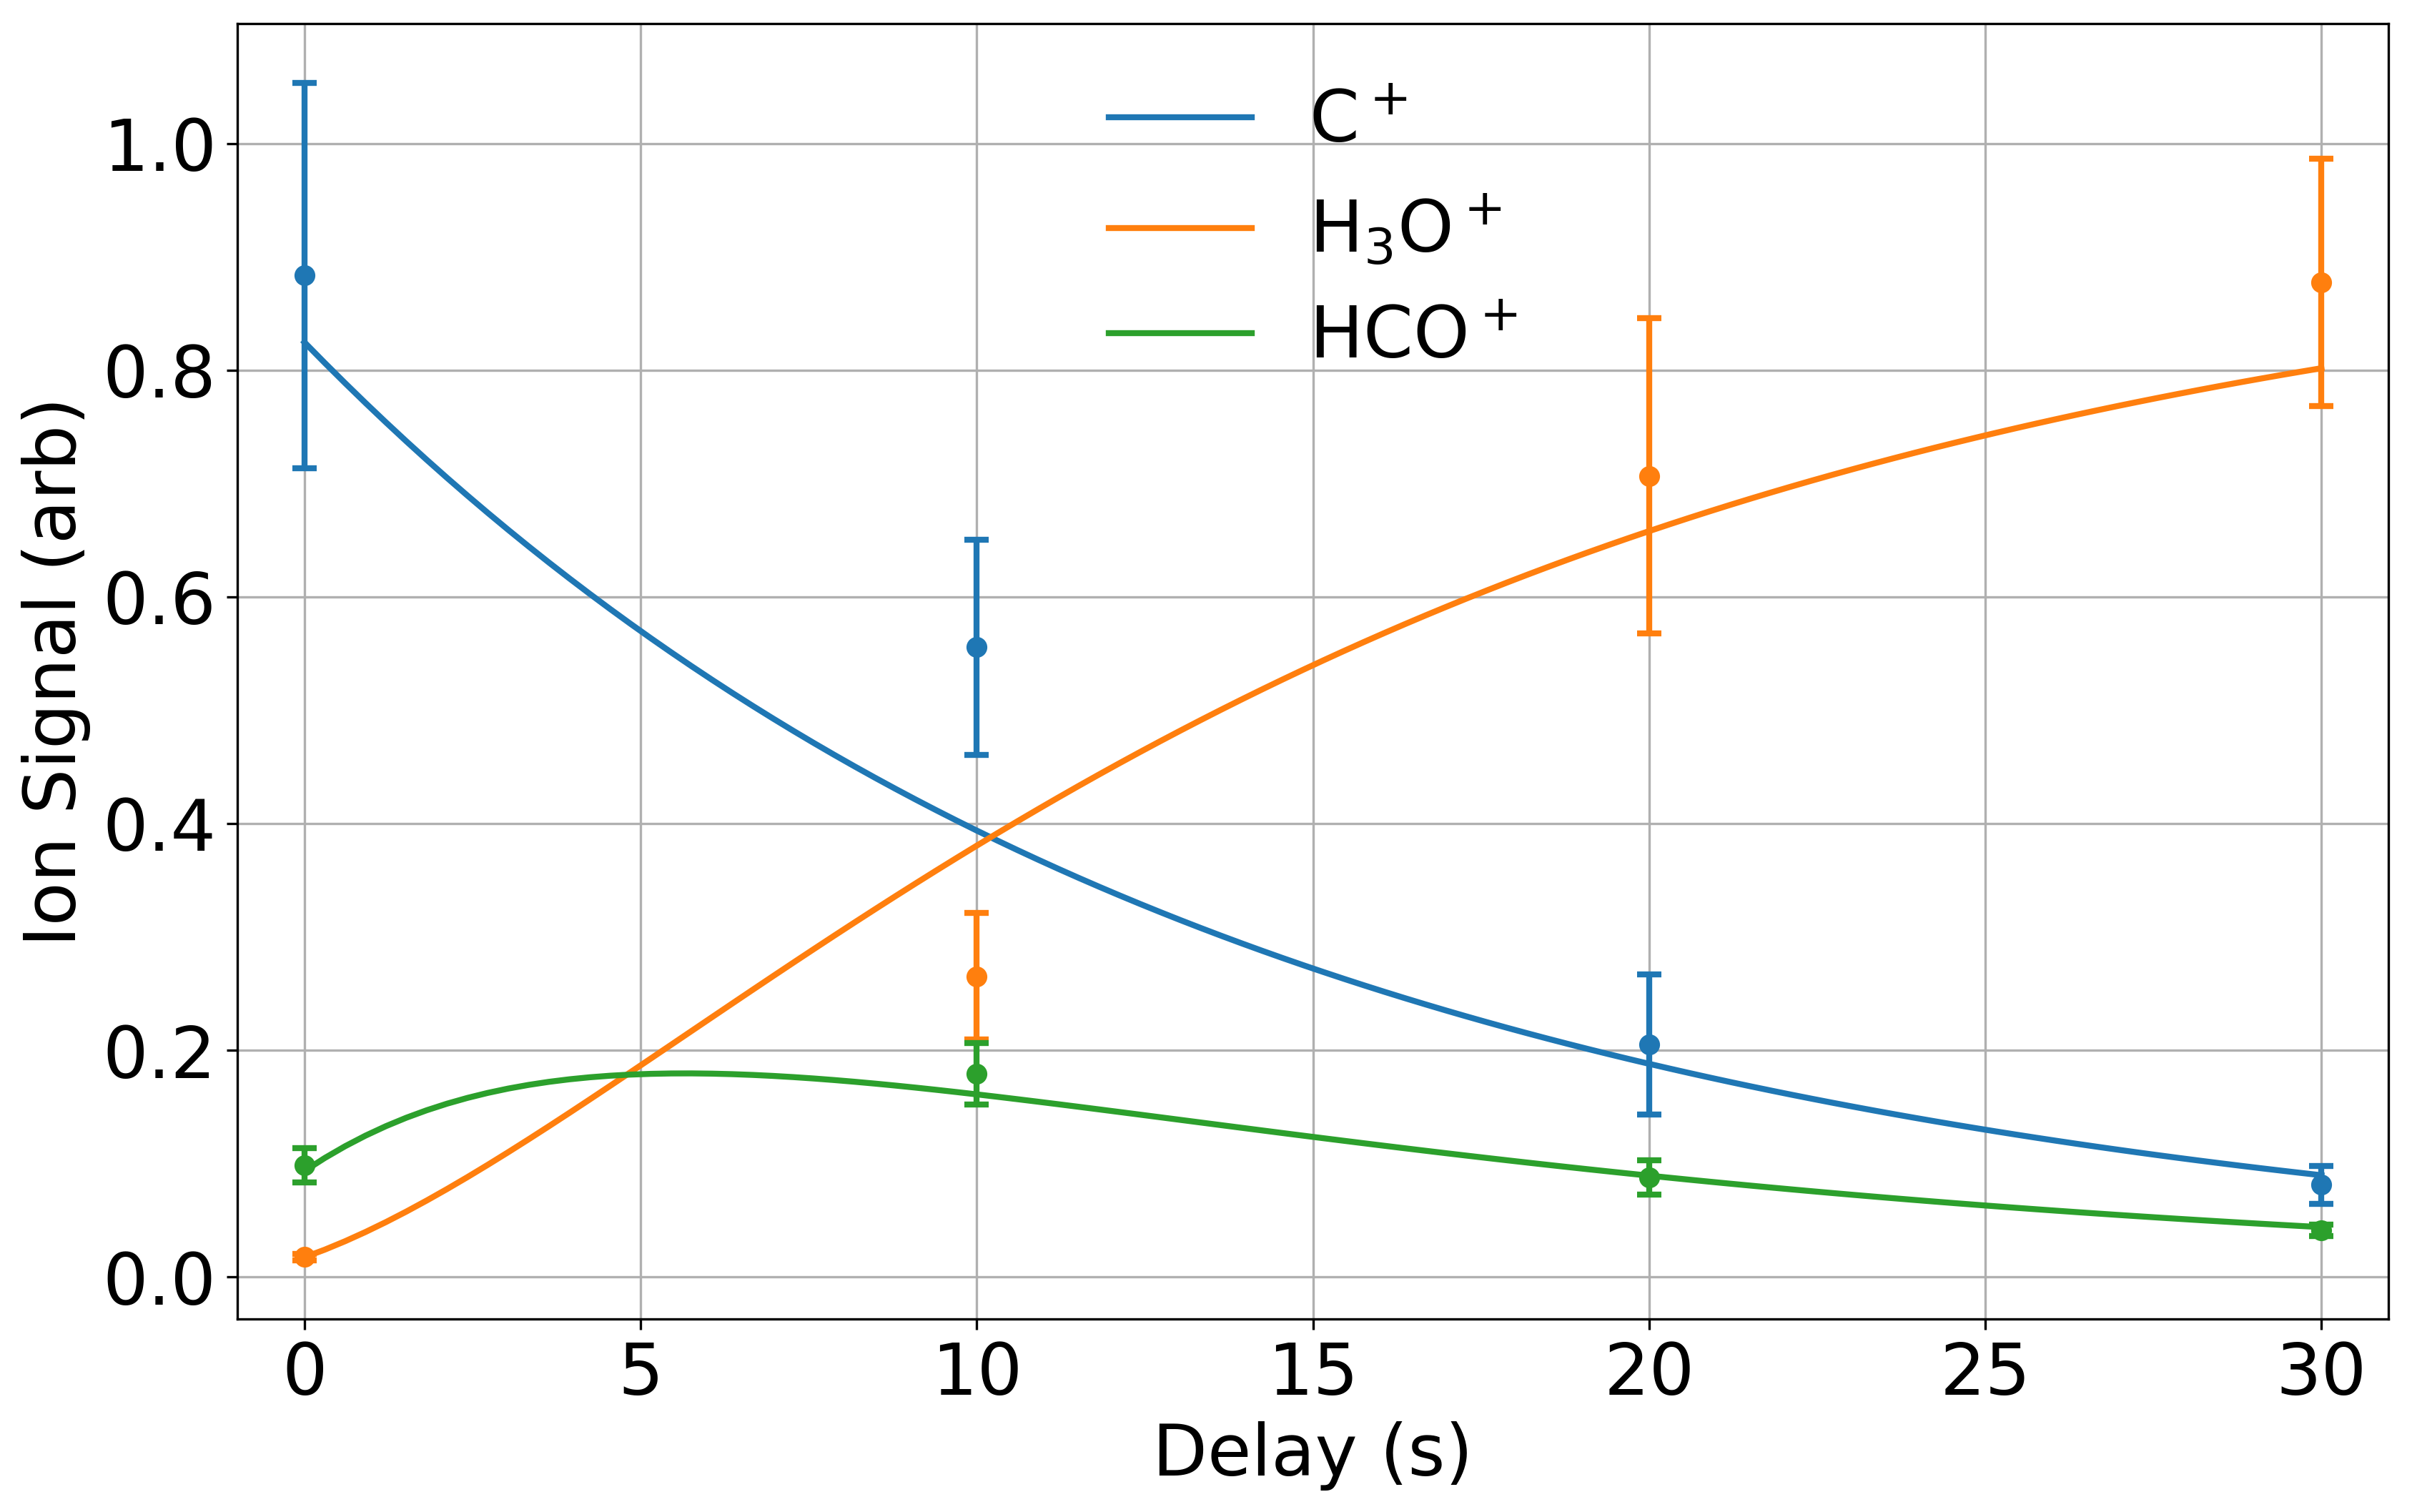
\includegraphics[width=0.8\textwidth]{images/C_H2O_CO_traces.png}
	\caption{text}
	\label{fig: HCO+H2O rate}
\end{figure}

\begin{figure}
	\centering
	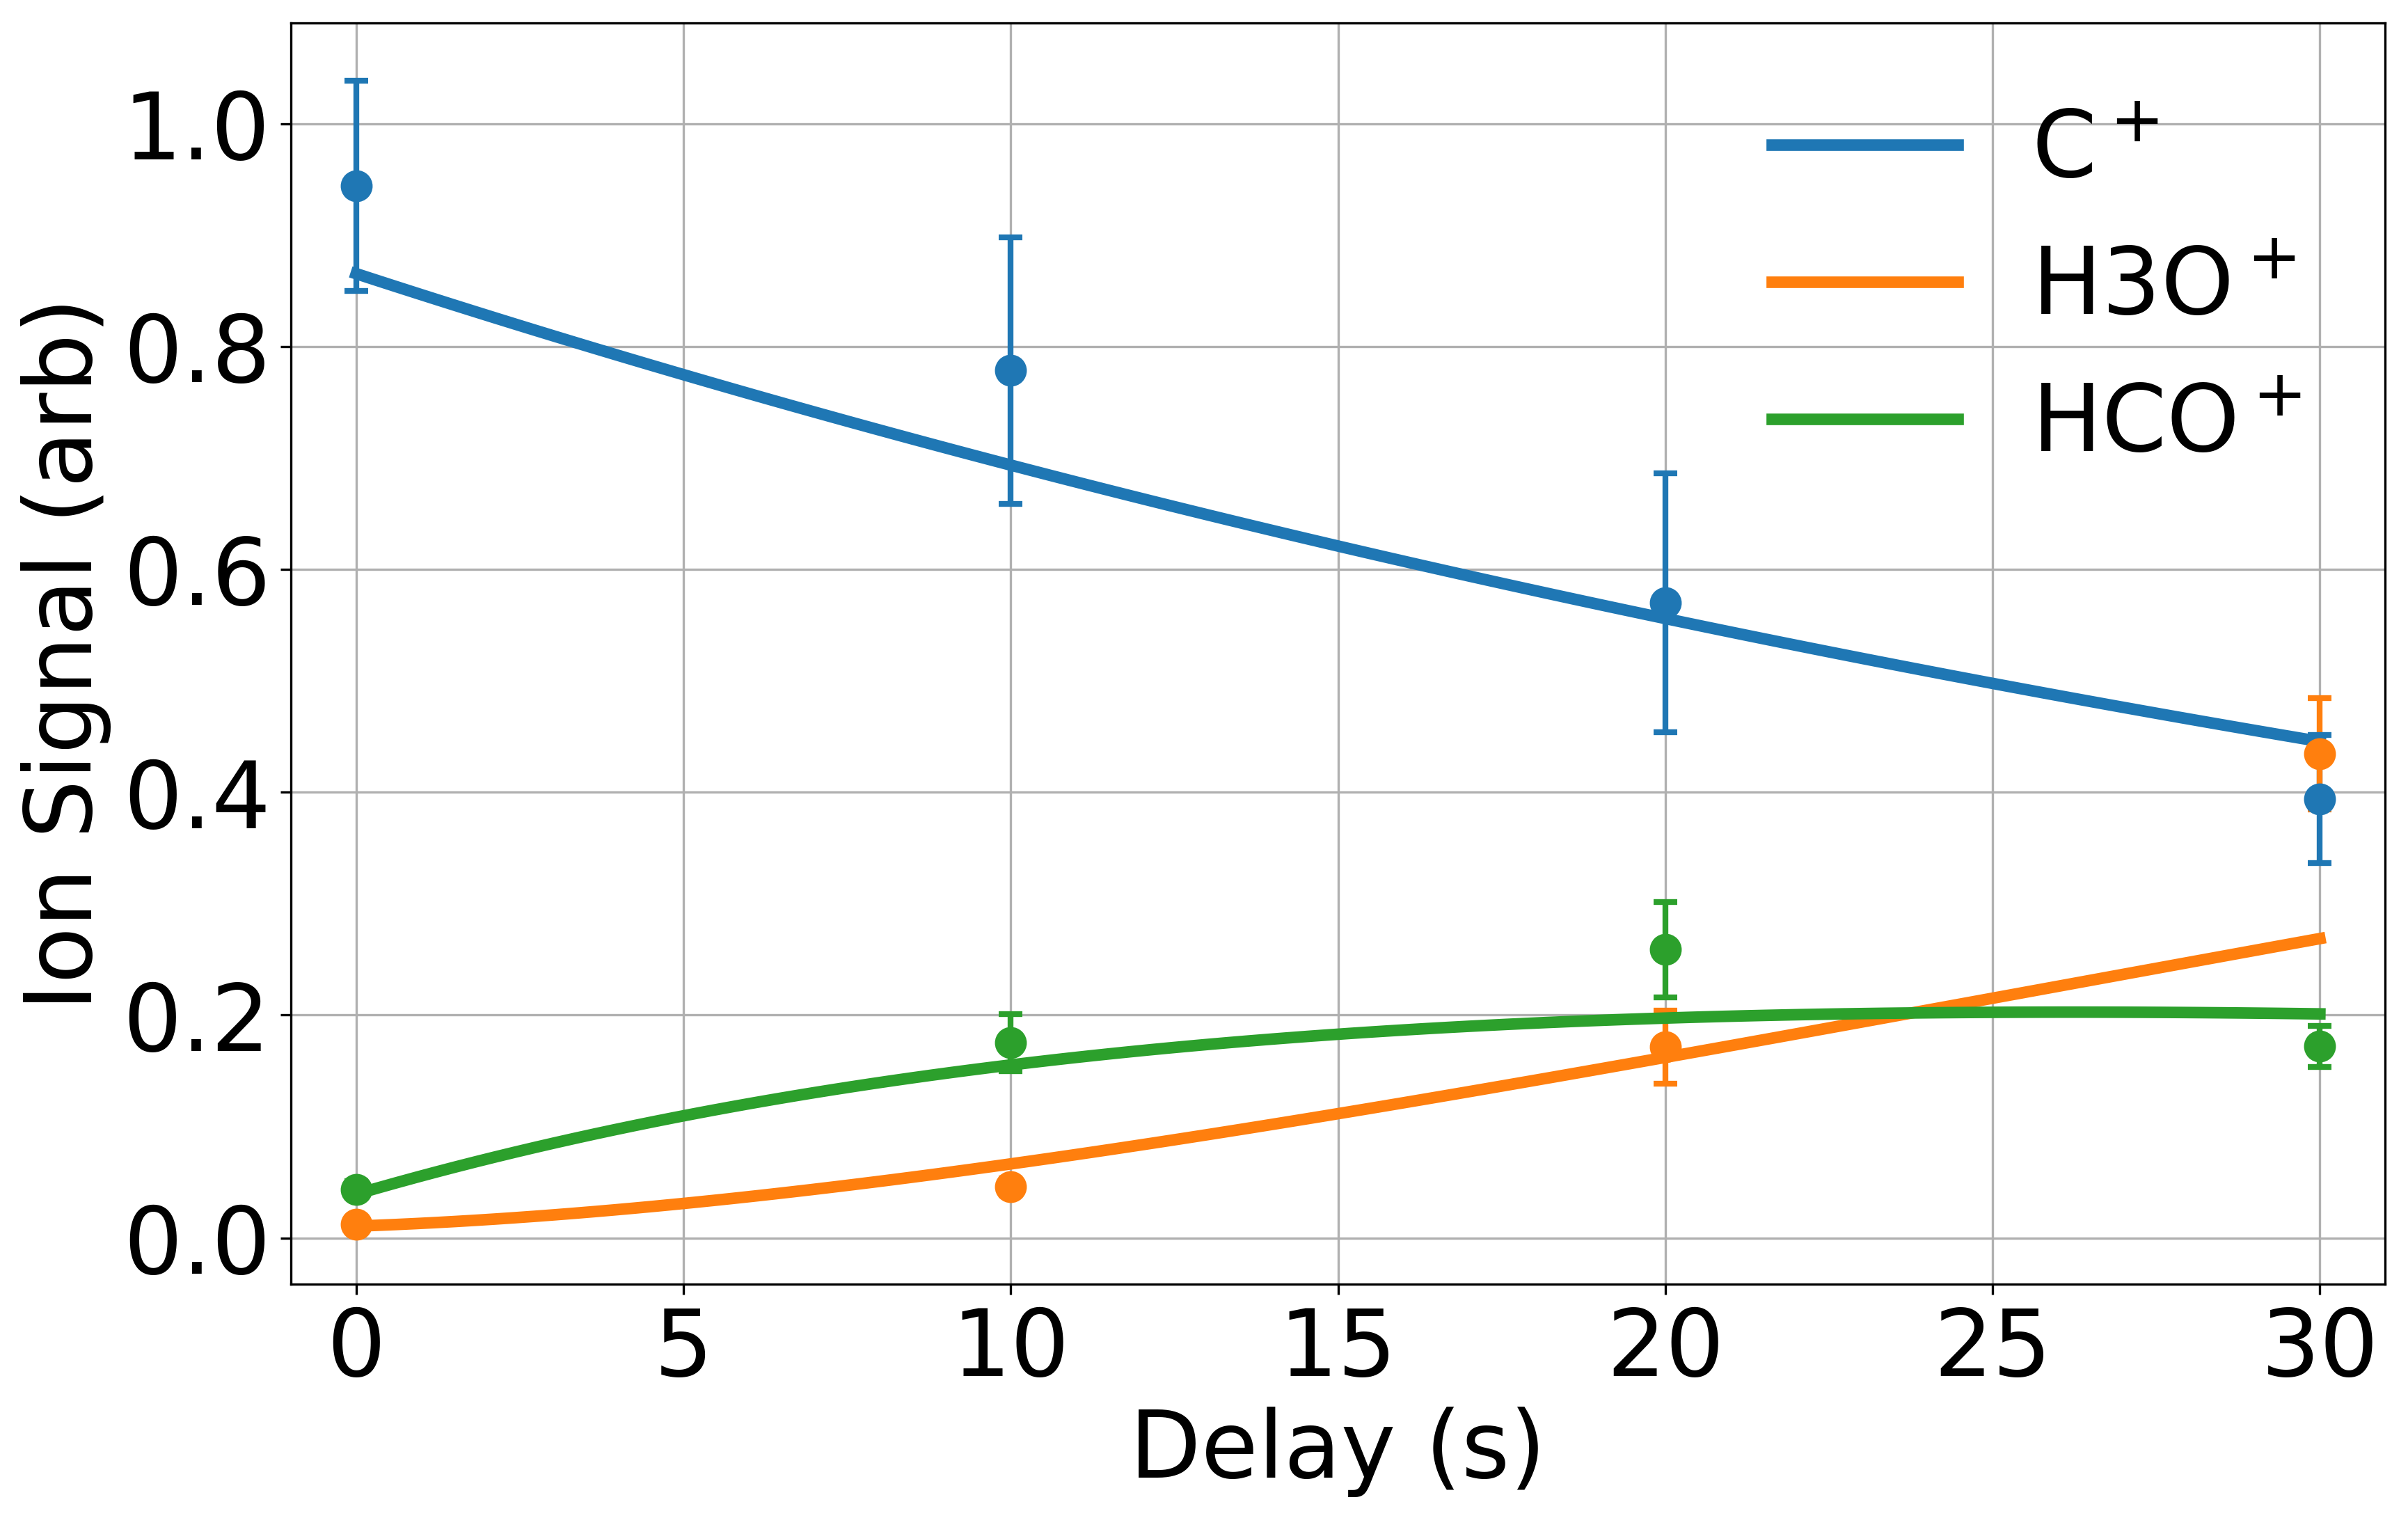
\includegraphics[width=0.8\textwidth]{images/C_H2O_beam_traces.png}
	\caption{text}
	\label{fig: [HCO]+H2O rate}
\end{figure}